\documentclass[m,bachelor,binding,twoside,palatino]{WeSTthesis}

  \usepackage[
    backend=biber,
    style=numeric-comp,
    url=false,
    doi=false,
    isbn=false
  ]{biblatex}
  \usepackage{graphicx}
  \usepackage{mathtools}
  \usepackage{float}
  \usepackage{amssymb}
  \usepackage{amsmath}
  \usepackage{rotating}
  \usepackage[ngerman,english]{babel}
  \usepackage[utf8]{inputenc}           % correct input encoding
  \usepackage[T1]{fontenc} 				% correct output encoding
  \usepackage{booktabs}

  \selectlanguage{\ngerman}
  \addbibresource{BAZitate.bib}
  
  \newcommand{\vect}[1]{\textbf{#1}} 
  \newcommand{\mat}[1]{\textbf{\MakeUppercase{#1}}}

  \renewcommand{\arraystretch}{1.3}
  \newcommand{\ra}[1]{\renewcommand{\arraystretch}{#1}}
\begin{document}


\title{\textbf{Vorhersage von Gefechts-Ausgängen im Echtzeit-Strategiespiel StarCraft II mittels Convolutional Neural Networks}}

\author{Frank Schaust}

\degreecourse{Informatik}

\firstreviewer{Prof.\ Dr.\ Steffen Staab}
\firstreviewerinfo{Institute for Web Science and Technologies}

\secondreviewer{}
\secondreviewerinfo{Institute for Web Science and Technologies}

\maketitle

\section{Motivation}

Das Thema der Bachelorarbeit ist die Adaption von Machine Learning (zu Deutsch: Maschinelles Lernen) Algorithmen zur Vorhersage von Gefechts-Ausgängen zweier feindlicher Armeen in dem Echtzeit-Strategiespiel StarCraft II. Das Ziel der Arbeit ist die Untersuchung, ob existierende Image Classification (zu Deutsch: Bildklassifikation) Algorithmen für komplexe Aufgaben in einer atypischen Domäne genutzt werden können. Kernbestandteil ist daher der Vergleich bestehender Architekturen auf dieser neuen Domäne. Die Domäne unterscheidet sich von konventionellen Bildformaten, da die Eingabedaten in Form von domänenspezifischen Eigenschaftsmatrizen vorliegen. Es werden vorwiegend Convolutional Neural Networks (folgend CNN, zu Deutsch etwa: Faltende Neuronale Netze) genutzt um Matrix-Repräsentationen von Spielzuständen zu verarbeiten und auf Grundlage derer den Ausgang der Kampfszenarien vorherzusagen. 

CNNs sind eine Machine Learning Methode, die unter anderem von den Gewinnern der ImageNet Large Scale Visual Recognition Challenge \textit{GoogLeNet} \parencite{DBLP:journals/corr/SzegedyLJSRAEVR14} genutzt wurde. In diesem Aufgabenfeld konnten CNNs im Vergleich zu anderen Image Classification Verfahren gute Resultate erzielen. Außerdem fanden CNNs in der Vergangenheit erfolgreich Anwendung in anderen Forschungsgebieten, welche keinen direkten Bezug zu Image Classification hatten, wie zum Beispiel bei der Entdeckung von medizinischen Wirkstoffen (AtomNet \parencite{DBLP:journals/corr/WallachDH15}).

Gefechte in StarCraft II bestehen aus zwei oder mehr Armeen. Jede Armee wird von einem unterschiedlichen Spieler kontrolliert, dessen Ziel es ist mit den Fähigkeiten seiner eigenen Einheiten sämtliche Einheiten des Gegners zu zerstören. Gefechte beinhalten komplexe Interaktionen, da jede Einheit ihre Position auf dem Schlachtfeld ändern und feindliche Einheiten angreifen und schlussendlich zerstören kann. Erfahrene menschliche Spieler können Gefechts-Ausgänge solcher Aufeinandertreffen im Allgemeinen mit einer angemessenen Wahrscheinlichkeit vorhersagen.

Um den Zustand des Spiels darzustellen werden Matrix-Repräsentationen genutzt. Jede Matrix repräsentiert einen anderen Aspekt (wie zum Beispiel Einheiten-Gesundheit, Einheiten-Typ, usw.) des Spiel-Zustandes in Bezug auf die Position auf dem Spielfeld. Gefechts-Vorhersage kann als Image Classification Aufgabe gesehen werden, da die genutzten Matrizen in einer ähnlichen Form klassifiziert werden können wie Bilder. Es werden Matrizen als EIngabe genutzt und es werden diskrete Werte als Ausgabe erhalten. Der Unterschied zwischen Bildern und Matrix-Repräsentation ist, dass jedes Bild explizit ein  oder mehrere Objekte zeigt, welche klassifiziert werden, während jede Matrix-Repräsentation eine implizierte Bedeutung hat. Die impliziten Bedeutungen zu lernen und zu kombinieren ist eine interessante Aufgabe für eine CNN-Architektur.

Der Versuch das Verhalten von Computerspielen vorherzusagen ist interessant, weil sie eine hervorragende Umgebung bieten um die Leistungsfähigkeit von Machine Learning Methoden zu testen. Sie stellen eine kontrollierbare Menge an Umweltfaktoren bereit -- im Fall von StarCraft~II die Anzahl der Einheiten, ihre Positionen und Kampfstärke -- welche genutzt werden kann um beliebig viele Trainingsdaten von kontrollierbarer Schwierigkeit zu erzeugen. Der Zustand des Spiels und der Ausgang des Gefechts sind klar zu bemessen und es gibt konkrete Regeln, die der Algorithmus lernen muss, um zuverlässige Vorhersagen zu treffen, wie zum Beispiel: \textit{Ein Marine greift mit X Schadenspunkten an}, oder \textit{Wenn die Lebenspunkte einer Einheit auf 0 oder tiefer fallen, stirbt sie}. Die Schwierigkeit für den Algorithmus liegt darin die richtigen Schlüsse zu ziehen, ohne explizites Wissen über die zugrundeliegenden Regeln des Spiels zu haben. Neben der Eignung als Machine Learning Problem, wird ein erfolgreicher Vorhersage-Algorithmus benötigt um künstliche Intelligenzen (KIs) für StarCraft~II zu implementieren. Damit KIs das Spiel auf einem hohen Niveau spielen können, müssen sie in der Lage sein, den Ausgang eines Gefechtes vorherzusagen um abzuwägen, ob sie den Kampf eingehen können, oder den Rückzug wählen müssen. 

In dieser Bachelorarbeit werden die betreffenden theoretischen Grundlagen für diese Problemstellung in Sektion \ref{th} zusammengetragen. Zudem liefert Sektion \ref{SC2} eine formalisierte Darstellung der Spielumgebung von StarCraft~II. Verwandte Arbeiten wurden auf mögliche Beiträge zu diesem Thema analysiert und in Sektion \ref{VerwandteArbeiten} zusammengefasst. Es wurde ein Framework geschaffen, welches basierend auf dem in StarCraft~II enthaltenen Map-Editor die Generierung beliebig vieler Trainingsdaten sowohl in Form von Spieldaten in Matrix-Repräsentation als auch als Screenshots in gängigen Bildformaten ermöglicht. Das Framework wird in Sektion \ref{datagen} genauer beschrieben. Zudem wurden bestehende Architekturen für die fallspezifischen Eingabematrizen adaptiert. Die genutzten Architekturen werden in Sektion \ref{Archs} genauer beschrieben und in Sektion \ref{Resultate} analysiert und verglichen. 

\subsection{StarCraft~II}
\label{SC2}

StarCraft~II ist ein Echtzeit-Strategiespiel entwickelt und veröffentlicht von Blizzard Entertainment. Es ist überwiegend deterministisch\footnotemark und das Ziel ist es alle feinlichen Einheiten auf einer Karte zu vernichten ohne selbst dabei vernichtet zu werden.  

Zu Beginn eines jeden Spiels kann der Spieler zwischen drei Rassen wählen. Jeder Spieler kontrolliert eine Menge an Einheiten U = \{$u_1, u_2, ... u_n$\}.

Das Spiel läuft im Allgemeinen in Echtzeit ab, kann allerdings auf Zeitschritte abstrahiert werden, wo in jedem Zeitschritt die gegebenen Befehle den kommenden Zeitschritt beeinflussen. Daher kann der Spielablauf als eine diskrete Serie von Zuständen repräsentiert werden. Intern läuft das Spiel mit einer Rate von 20 Zuständen pro Sekunde. 

\footnotetext{Die hauptsächlichen Quellen für Zufälligkeiten sind laut DeepMind \textit{Angriffsgeschwindigkeit} und \textit{Aktualierungsreihenfolge}. Diese Zufälligkeiten können durch das manuelle setzen eines Zufallswertes ausgemerzt werden  \parencite{DBLP:journals/corr/abs-1708-04782} und in die Berechnungen eingearbeitet werden.}

Jede Einheit besitzt eine allgemeine Beschreibung die ihr einen Typ $t(u_i)$ zuweist. $t(u_i)$ kann einer von drei Typen sein $t(u_i) \in$ \{ Bodeneinheit, Lufteinheit, kleine Bodeneinheit \}. Zusätzlich kann jede Einheit mit zwei weiteren Attributen $at(u_i)$, $st(u_i)$ versehen werden, die ihre weiteren Eigenschaften spezifizieren. Eine Einheit kann eine leichte oder eine gepanzerte Einheit sein ($at(u_i)$) und außerdem dem biologischen oder mechanischen Typ angehören ($st(u_i)$). Es gibt vereinzelt Ausnahmen in denen Einheiten keinem Typ oder beiden Typen angehören.

Einheiten bewegen sich auf einer 2D Karte und können in Abhängigkeit von der Zeit einer Position zugeordnet werden. Die Karte kann als Matrix mit Dimensionen $H \times B$, $H,B \in \mathbb{N}$ definiert werden, wodurch die Position einer Einheit als zweidimensionaler Punkt $p^t(u_i)$ = $(x,y)$ verstanden werden kann, bei dem $t$ die Spielzeit darstellt und $x \leq B, y \leq H$ gilt.

Jede Einheit verfügt über ein Attribut Lebenspunkte $hp^t(u_i)$, eine Bewegungsrate $mr(u_i)$ und eine Sichtweite $sr(u_i)$. Lebenspunkte sind von der Spielzeit abhängig und können sich während dem Verlauf des Spiel ändern. Wenn $\exists t$ indem $hp^t(u_i) \leq 0$ gilt, so wird die Einheit for alle folgenden Zeitschritte $t' > t$ als tot behandelt und ist nicht mehr in der Lage ins Spielgeschehen einzugreifen. Die Bewegungsrate bestimmt wie schnell sich eine Einheit über die Spielkarte bewegen kann. Die Sichtweite bestimmt den Radius um eine freundliche Einheit herum in dem die Karte aufgedeckt wird. Ein Spieler kann nur jene gegnerischen Einheiten sehen, welche sich im Sichtbereich von mindestens einer freundlichen Einheit aufhalten. Zusätzlich verfügen Einheiten über weitere Attribute, welche ihre Kampfstärke definieren: Schaden $d(u_i)$, Abklingzeit $cd(u_i)$ und Waffenreichweite $wr(u_i)$. Der Schadenswert wird genutzt um den Schaden zu berechnen, den eine Einheit mit einem einzelnen Schuss verursacht. Abklingzeit bestimmt wie lange eine Einheit warten muss bevor sie einen weiteren Schuss abgeben darf und wird in Sekunden bemessen. Die Waffenreichweite ist der Radius eines Kreises in dessen Fläche die Einheit Angriffe ausführen kann. Der Mittelpunkt des Kreises ist immer die Position der Einheit. 

Das Schadensattribut kann durch eine Menge an möglichen Zieltypen $tt(u_i)$ erweitert werden. Eine Einheiten können zum Beispiel lediglich Bodeneinheiten angreifen, während andere nur Lufteinheiten angreifen können. Daher kann die Menge der angreifbaren Einheiten $tu(u_i)$ definiert werden als Menge aller gegnerischen Einheiten $EU$ für die gilt: \{$x \in EU : t(x) \in tt(u_i)$\}. Einige Einheiten verfügen außerdem über ein Attribut Bonusschaden $bd^{at}(u_i)$, welches auf dem at-Attribut der attackierten Einheit beruht. Die Angriffe von Einheiten können zusätzlich verbessert werden, indem man bei den Einheiten die Verbesserungen ausbildet. Für jede Angriffsverbesserung erhält die Einheit einen Bonus von $d(u_i) \div 10$ - jedoch mindestens 1 - auf ihren Schaden. 

Viele Einheiten sind in der Lage Fähigkeiten $ab(u_i)$ zu nutzen. Die Fähigkeiten unterscheiden sich in ihren Effekten und Nutzungsmöglichkeiten. Einige können aktiv und manuell vom Spieler eingesetzt werden, andere sind passiv oder werden von bestimmten Konditionen im Spiel ausgelöst. Zauber sind eine besondere Form der Fähigkeiten und kosten die Einheiten Energie. Obwohl die intelligente Nutzung von Fähigkeiten und Zaubern in Mensch-gegen-Mensch Gefechten eine signifikante Rolle spielen, werden sie in dieser Arbeit vernachlässigt, da sie den simulierten Armeekommandeuren die Fähigkeit des automatisierten Lernens abverlangen würden. 
\section{Theoretischer Hintergrund}
\label{th}
In dieser Sektion werden wichtige Grundlagen definiert und anhand von Beispielen erl\"autert. Zun\"achst folgt eine Einf\"uhrung in Artificial Neural Networks (zu Deutsch: \textit{Künstliche neuronale Netze}) in Sektion \ref{ann}. Daraufhin werden Convolutional Neural Networks (zu Deutsch etwa:\textit{Faltende neuronale Netze}) und ihre allgemeinen Bestandteile n\"aher erkl\"art (Sektion \ref{cnn}). 

\subsection{Artificial Neural Networks}
\label{ann}
Artificial Neural Networks (ANNs) sind im Machine Learning (zu Deutsch: \textit{Maschinelles Lernen}) angewandte Techniken, die von biologischen neuronalen Netzen inspiriert sind.  

Machine Learning ist ein Bereich der Informatik, in dem man Probleme durch Algorithmen l\"osen m\"ochte, welche keinen statisch programmierten L\"osungweg ben\"otigen. Das Ziel von Machine Learning ist das Konstruieren von Algorithmen, die anhand von Datens\"atzen Schlussfolgerungen ziehen k\"onnen und bei Eingabe unbekannter Daten diese Schlussfolgerungen zur Vorhersage von Ergebnissen generalisieren k\"onnen.

ANNs k\"onnen als gerichtete Graphen verstanden werden. Sie bestehen aus einer Menge an Knoten mit einer Menge an Kanten als Verbindungen zwischen den Knoten, welche die Aktivierungen der Knoten transportieren. Bei ANNs wird zwischen verschiedenen Strukturen unterschieden. In dieser Arbeit werden ausschlie\ss{}lich sogenannte feed-forward neural networks (zu deutsch etwa: \textit{vorw\"arts gekoppelte neuronale Netze}) genutzt. In feed-forward neural networks sind Knoten in Layern (zu Deutsch: \textit{Schichten}) angeordnet, welche untereinander kommunizieren. Die Knoten in einem Layer senden somit Signale an Knoten in anderen Layern, k\"onnen allerdings keine Signale an Knoten des selben Layers senden. Des weiteren zeichnen sich feed-forward neural networks dadurch aus, dass ein Knoten eine Aktivierung immer nur zu dem Layer weitersendet, welcher als sein Nachfolger definiert ist. Es werden keine Aktivierungen an die voranstehenden Layer zurückgesendet. 

Neuronen in ANNs haben einen Bias und jede Verbindung zu anderen Neuronen ist mit einem Gewicht belegt. Die Werte beider Eigenschaften sind variabel und werden im Verlauf des Lernprozesses immer wieder angepasst. Au\ss{}erdem verf\"ugt jedes Neuron über eine Aktivierungsfunktion, welche die Ausgabe des Neurons abhängig vom Eingabewert definiert.

%Artificial neurons are assigned with a bias and connections between neurons have a weight assigned to them. Additionally, neurons have an activation function. An activation function defines the output of a node dependent on the given input. The output function is a function, that takes the computed activation and returns the final output, that is send to the next neuron. Artificial neurons are typically organized in layers. Those layers can perform different kinds of transformations of their inputs (e.g. pooling layers, convolutional layers, etc. when looking at CNNs). 



Bild \ref{fig:basictop} zeigt eine einfache Topologie eines ANNs. Eine Eingabe wird vom Input Layer (zu Deutsch: \textit{Eingabeschicht}) in den Hidden Layer (zu Deutsch: \textit{Versteckte Schicht}) gegeben und von diesem in die letzte Schicht, welche als Output Layer (zu Deutsch: \textit{Ausgabeschicht}) funktioniert weitergereicht. 

\begin{figure}[ht]
\centering
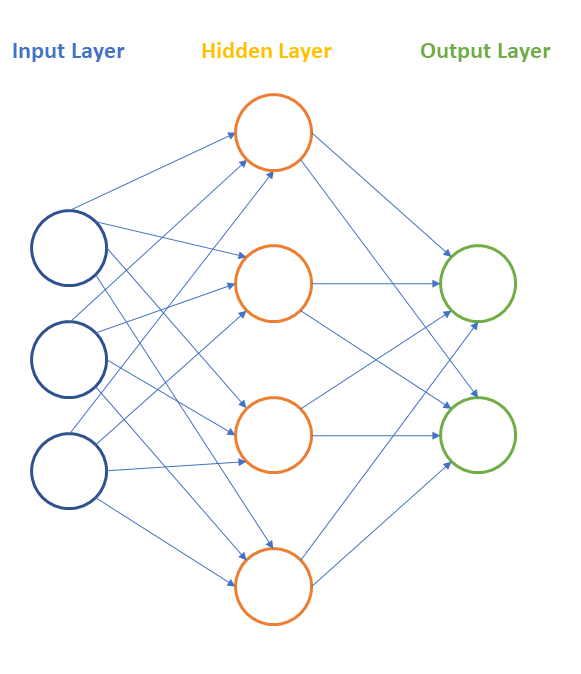
\includegraphics[scale=0.5]{pictures/grafiken/Folie3}
\caption[Caption for LOF]{Topologie eines einfachen ANNs.} 
\label{fig:basictop}
\end{figure}

Neural Networks (zu Deutsch: \textit{Neuronale Netze}) können als mathematische Modelle verstanden werden, welche eine Funktion $f : X \rightarrow Y$ definieren. In einem Neural Network wendet jedes Neuron eine Funktion auf seine Eingangswerte an, bevor es diese zur n\"achsten Schicht sendet. Somit kann die Funktion eines Neural Networks als eine Komposition aus jeder sich im Networks befindlichen Funktion definiert werden. 

Bezogen auf Bild \ref{fig:composedGraph}, sieht die zusammengesetzte Funktion des Networks wie folgt aus: 
\begin{equation}
\label{eq:compf}
f(g_1(h_1(x), h_2(x)),g_2(h_2(x), h_3(x)))
\end{equation}

\begin{figure}[ht]
\centering
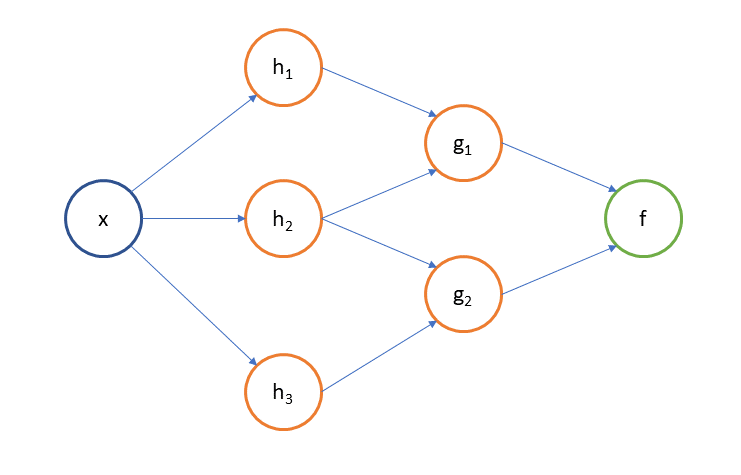
\includegraphics[scale=0.4]{pictures/grafiken/Folie4}
\caption[Caption for LOF]{Grafische Darstellung der zusammengesetzten Funktion $f$ aus Gleichung \ref{eq:compf}.}
\label{fig:composedGraph}

\end{figure}

\paragraph{Fully-connected layer}
Jeder Layer in einem klassischen ANN ist ein fully-connected Layer (zu Deutsch etwa: \textit{vollständig verbundene Schicht}). Neuronen in fully-connected Layern besitzen Verbindungen zu allen Neuronen des vorrangigen Layers. Jedes Neuron berechnet einen Ausgabewert $F(x)$ unter Verwendung des Eingabewertes \vect{x}, der Gewichte \mat{W}, die den Verbindungen zu dem vorherigen Layer zugewiesen sind, und eines Bias \vect{b}, der dem entsprechenden Neuron zugewiesen ist. 
\begin{equation}
\label{eq:fcl}
\begin{bmatrix}
w_{11} & ... & w_{1m}\\
. &  & .\\
. & . & .\\
. &  & .\\
w_{n1} & ... & w_{nm} 
\end{bmatrix} \cdot
\begin{bmatrix}
x_1\\
.\\
.\\
.\\
x_m
\end{bmatrix} + 
\begin{bmatrix}
b_1\\
.\\
.\\
b_n
\end{bmatrix} = 
\begin{bmatrix}
y_1\\
.\\
.\\
y_n
\end{bmatrix}
\end{equation}
Gleichung \ref{eq:fcl} zeigt die allgemeine Formel nach welcher der Ausgabewert eines fully-connected Layers berechnet wird. $n$ steht für die Anzahl der Neuronen im Layer und $m$ ist die Anzahl der Eingabewerte des vorherigen Layers. Die Gleichung kann auch wie folgt in Vektornotation formuliert werden: 
\begin{equation}
\label{eq:VecNot}
F(\vect{x}) = (\mat{W} \cdot \vect{x}) + \vect{b}^T
\end{equation} 
In Gleichung \ref{eq:VecNot} sind \mat{W} und \vect{b} lernbare Parameter, welche vom Optimierungsalgorithmus abgepasst werden k\"onnen. Sie stehen in der Gleichung f\"ur die Gewichte(\mat{W}) und den Bias(\vect{b}) des entsprechenden Layers.

\paragraph{Rectified Linear Units Layer}

In ANNs finden eine Vielzahl von Aktivierungsfunktionen Anwendung. Im Folgenden wir die ReLU-Funktion vorgestellt, da sie in den Modellen, die in dieser Arbeit implementiert werden genutzt wird. Sie ist wie folgt definiert: $relu(x) = max(0, x)$. Die Aktivierungsfunktion wird nach der Verarbeitung eingehender Werte im Neuron auf das Ergebnis angewandt und entfernt negative Werte aus dem Ausgabevektor des Neurons, bevor der Vektor an das n\"achste Layer weitergereicht wird \parencite{Wu.2017}.

\paragraph{Normalization Layer}

Das Normalization Layer (zu Deutsch: \textit{Normalisierungsschicht}) wird zur Normalisierung der Aktivierungen des vorherigen Layers genutzt. Nachfolgend wird ausschließlich batch normalization(BN) genutzt, da es sowohl f\"ur fully-connected Layer als auch f\"ur convolutional Layer genutzt werden kann und die Trainingsgeschwindigkeit des Netzwerks beschleunigt \parencite{DBLP:conf/icml/IoffeS15}.

\paragraph{Loss Function}

Die Loss Function (zu Deutsch: \textit{Verlustfunktion}) evaluiert wie genau ein Neural Network die ground-truth (zu Deutsch etwa: Grundwahrheit) der Trainingsdaten vorhersagt. Ihre Aufgabe besteht darin den Abstand zwischen der ground-truth \vect{(x, y)} einer Eingabe \vect{x} und der Vorhersage des ANNs $\hat{y}$. Neural Networks versuchen Gewichte und Biase so anzupassen, dass dieser Wert minimiert wird. Ein Beispiel f\"ur eine Loss function $z$ w\"are \parencite{Wu.2017}:

\begin{equation}
z = \frac{1}{2}\|\vect{(x, y)} - \hat{y}\|^2
\end{equation}


\paragraph{Softmax-Funktion}

Die Softmax-Funktion ist eine Variante der logisitschen Funktion. Die Funktion erh\"alt einen Vektor \vect{z} mit reellen Werten und einer beliebigen Dimension $K$ und verrechnet dessen Werte, so dass sich jeder Wert des Vektors \vect{z} im Bereich (0, 1] befindet und die Summe aller Werte 1 ergibt. Die Softmax-Funktion wird nach folgender Formel berechnet \parencite{Goodfellow-et-al-2016}:

\begin{equation}
softmax(\vect{z})_j = \frac{\mathrm{e}^{z_j}}{\sum_{k=1}^K \mathrm{e}^{z_k}}
\end{equation}
\\

Eine vollständige Funktion f\"ur das in Bild \ref{fig:basictop} gezeigte ANN w\"are:
\begin{multline*}
f(\mathbf{x}) = softmax(\mathbf{W_2} \cdot relu(\mathbf{W_1} \cdot \mathbf{x} + \mathbf{b_1}) + \mathbf{b_2} )
\end{multline*}


Der Eingabevektor \vect{x} ist in $\mathbb{R}^3$. Zuerst, wird \vect{x} vom Hidden Layer verarbeitet. In diesem Beispiel ist der Hidden Layer fully-connected, so dass die Formel f\"ur fully-connected Layer \ref{eq:fcl} mit $\mathbf{W_1}$ und $\mathbf{b_1}$ angewendet werden kann. $\mathbf{W_1}$ ist eine $4 \times 3$ Matrize und $\mathbf{b_1}$ ist in $\mathbb{R}^4$. Das Resultat wird mit einer Aktivierungsfunktion - in diesem Fall der ReLU-Funktion - verechnet und hat danach die Dimension $4\times1$. Daraufhin wird das Resultat an den Output Layer weitergegeben, welcher auch ein fully-connected Layer ist. Auch hier wird Gleichung \ref{eq:fcl} f\"ur fully-connected mit $\mathbf{W_2}$ als $2\times4$ Matrix und $\mathbf{b_2}$ als Vektor in $\mathbb{R}^2$ angewandt. Zuletzt wird die Softmax-Funktion auf das Ergebnis des Output Layers angewandt. Die Dimension des Ausgabevektors ist $2\times1$.


\subsection{Convolutional Neural Networks}

\label{cnn}

Ein Convolutional Neural Network (CNN) ist ein tiefes, feed-forward ANN. Es findet h\"aufig  Anwendung um Aufgaben im Zusammenhang mit Bildern, wie zum Beispiel Bildklassifikationen, zu l\"osen. Im Vergleich zu ANNs ben\"otigen CNNs im Allgemeinen weniger Gewichte, durch ihre Eigenschaft der lokalen Konnektivit\"at.

\"Ahnlich wie ANNs bestehen CNNs jeweils aus einem Input und einem Output Layer. Zwischen diesen beiden Layern befindet sich der Hidden Layer, in dem die Informationen aus den Eingabedaten haupts\"achlich verarbeitet werden. Der Hidden Layer kann aus verschiedenen Layer-Typen zusammengesetzt werden, welche beliebig untereinander kombiniert werden k\"onnen. Einige dieser Layer sind zum Beispiel: Convolutional, Pooling, fully-connected und Normalization Layer. In der Praxis sind ideale Layerzusammenstellungen stark an die Problemstellung gebunden und werden empirisch bestimmt. 

\paragraph{Convolutional layers}

Das Convolutional Layer ist einer der Kernbestandteile eines CNNs. Der Layer verf\"ugt \"uber einen Filter, bemessen durch einen Tensor des selben Ranges wie die Eingabedaten, welcher sogenannte Feature (zu Deutsch: \textit{Merkmale}) in den Eingabedaten detektiert. Filter sind durch ihre rezeptiven Felder charakterisiert, welche die Gr\"o\ss{}e der zeitgleich untersuchten Areale bestimmen \parencite{DBLP:journals/corr/OSheaN15}. Ein Beispiel f\"ur das rezeptive Feld eines Neurons k\"onnte eine $M \times N$ große Fl\"ache seine, welche kleinere oder gleich gro\ss{}e Abmessungen haben sollte wie die Dimensionen der Eingabedaten. Da die Tiefe des Filters $D_f$ \"aquivalent zu der Tiefe der Eingabedaten $D_i$ ist, ergibt sich $D_f = D_i$. Eingabewerte mit Dimensionen $10 \times 10 \times D_i$ w\"urde demnach in einem $M \times N \times D_i$ dimensionierten Filter mit $M, N \leq 10$ resultieren. 

Während der Filter die Eingabe verarbeitet, wird er \"uber die Eingabematrix geschoben und multipliziert die Werte in dem untersuchten Bereich mit den Werten seines Filters. Die Produkte werden zu einem einzigen Werte aufsummiert, welcher dann den Wert f\"ur das Areal widerspiegelt. Wenn der Prozess endet, ist das Ergebnis eine etwas kleinere Matrix, in welcher die aufsummierten Ergebnisse f\"ur jede m\"ogliche Position des Filters in den Eingabedaten erfasst sind. Aufbauend auf dem Beispiel im vorherigen Absatz ergibt sich eine Ausgabedimension von $6\times6$ bei einem $10\times10$ Eingabewert und einem $5\times5$ Filter. Im Allgemeinen resultiert eine Eingabe mit Bemessung $H^l \times W^l \times D^l$ und einem Filter der Gr\"o\ss{}e $H \times W \times D^l \times D$ in einer Ausgabe der Dimension $(H^l - H + 1) \times (W^l - W + 1) \times D$. In dieser Notation verweist $l$ auf den vorherigen Layer \parencite{Wu.2017}.

Sollte eine Ausgabe mit den selben Dimensionen wie die Eingabe ben\"otigt werden, so ist es m\"oglich \textit{padding} (zu Deutsch in etwa: \textit{Polsterung}) zu nutzen, um der Matrix Spalten und Zeilen nach Bedarf hinzuzuf\"ugen. Um die Dimensionen der Eingabematrix zu erhalten, m\"ussen $\lfloor \frac{H-1}{2} \rfloor$ Zeilen oberhalb der ersten Zeile und $\lfloor \frac{H}{2} \rfloor$ unterhalb der letzten Zeile hinzugef\"ugt werden. Außerdem m\"ussen $\lfloor \frac{W-1}{2} \rfloor$ Spalten vor der ersten Spalte und $\lfloor \frac{W}{2} \rfloor$ Spalten nach der letzten Spalte eingef\"ugt werden. Der Notation der vorangegangenen Abs\"atze folgend, beziehen sich $W$ und $H$ auf die vertikale und horizontale Dimension des Filters.

Zus\"atzlich kann ein \textit{stride}-Parameter (zu Deutsch: \textit{Schritt-Parameter}) $s$ definiert werden. Dieser Parameter bestimmt um wie viele Stellen der Filter nach jeder Rechnung auf der Matrix verschoben wird. Wenn jede m\"ogliche Position auf der Matrix evaluiert werden soll, betr\"agt der Wert des stride-Parameters $s=1$. F\"ur alle $s > 1$ wird der Filter $s - 1$ Positionen entlang beider Axen \"uberspringen.

Der Vorgang des "Abgehens" der Eingabewerte kann durch eine mathematische Formel [\ref{eq:convolution}] beschrieben werden. In der Formel ist der stride-Parameter $s=1$ und es findet kein padding statt. Die Notation folgt der bereits etablierten Notation und $H^{l+1}$, $W^{l+1}$ und $D^{l+1}$ beziehen sich auf H\"ohe, Breite und Tiefe der Ausgabematrix.
 
\begin{equation}
y \in \mathbb{R}^{H^{l+1} \times W^{l+1} \times D^{l+1}}
\end{equation}

mit $H^{l+1} = H^l - H + 1$, $W^{l+1} = W^l - W + 1$, and $D^{l+1} = D$ \parencite{Wu.2017}.


\begin{equation}
\label{eq:convolution}
y_{i',j',di} = \sum_{i=0}^{H}\sum_{j=0}^{W}\sum_{d =0}^{D^l} f_{i,j,d,di} \cdot x^{l}_{i'+i, j'+j, d}
\end{equation}

$f$ bezeichnet die Menge aller Filter und $x^l$ ist die Ausgabe des vorherigen Layers. Die Gleichung \ref{eq:convolution} wird \"uber die komplette Tiefe $D^l$ der Eingabe wiederholt ($0 \leq di \leq D^l$). Sie wird lediglich auf Positionen $(i',j')$ angewandt, welche die Bedingungen $0 \leq i' < H^{l + 1}$ und $0 \leq j' < W^{l + 1}$ erfüllen \parencite{Wu.2017}.

Im Bezug auf hoch dimensionierte Eingabewerte k\"onnen fully-connected neural networks r\"aumliche Abh\"angigkeiten nicht nutzen, da jedes Neuron vom jedem Neuron des vorherigen Layers Informationen sammelt und so immer alle Aktivierungen verarbeitet. Um r\"aumliche Informationen auszuwerten nutzen CNNs ein Pattern zur Erfassung lokaler Zusammenhänge. Aufgrund dieses Patterns, ist jedes Neuron nur mit einer kleinen Menge der Eingabegr\"o\ss{} verbunden. Hier wird nun das rezeptive Feld ben\"otigt, da es den Hyperparameter betitelt, welcher die r\"aumliche Bemessung des Sichtfeldes eines jeden Neurons abbildet.

\paragraph{Pooling layers}

Pooling Layer (zu Deutsch etwa: \textit{bündelnde Schicht}) werden auch als downsampling Layer bezeichnet. Ihre Aufgabe besteht darin die Ausgabewerte der vorherigen Layers in einen Wert zu kombinieren und somit die Dimensionen der weitergereichten Daten zu reduzieren. Bild \ref{fig:maxpool} zeigt eine bildliche Erkl\"arung des maxpool Layers.

\begin{figure}[H]
\centering
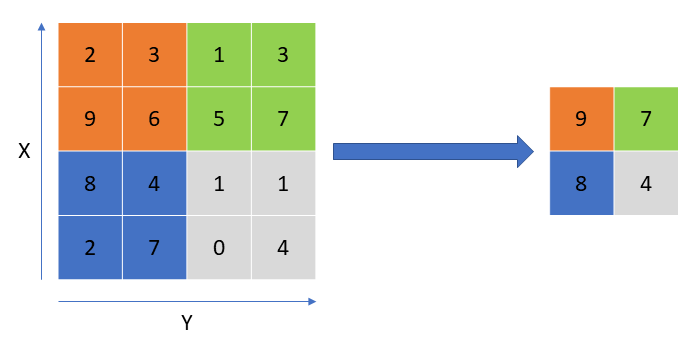
\includegraphics[scale=0.45]{pictures/grafiken/grafikenmax}
\caption[Caption for LOF]{Einfache Veranschaulichung des maxpool Layers mit $2 \times 2$ stride-Parameter.}
\label{fig:maxpool}

\end{figure}

Der maxpool Layer fu\ss{}t auf der Idee, dass die exakte Position eines Merkmals nicht so wichtig ist, wie seine Position in Relation zu anderen Merkmalen. Abh\"angig von der gestellten Aufgabe k\"onnte die Lage des Merkmals auch gar nicht relevant sein und die wichtige Information, die dieses Merkmal enth\"alt ist lediglich seine Existenz. Ein pooling Layer reduziert die Dimensionen der Eingabe in Abh\"angigkeit von seinen Parametern. So reduziert ein $2\times$ pooling Layer eine $8\times8$ dimensionierte Eingabe auf die Dimension $4\times4$, da es die Eingabematrix in sich nicht \"uberlappende $2\times2$ Quadrate unterteilt und f\"ur jedes Quadrat einen Wert errechnet, welcher in die Ausgabematrrix einflie\ss{}t. Die Inhalte der Ausgabe h\"angen von dem Typ des Layers ab, so errechnet ein maxpooling Layer immer die gr\"o\ss{}ten Werte beobachteten Bereichs, ein average-pooling Layer wiederum berechnet den Durchschnitt aller Werte in dem relevanten Bereich.

Der pooling Layer arbeitet auf der kompletten Tiefe der Eingabe und reduziert diese daher nicht, sondern berechnet jede Matrix unabh\"angig von den anderen. Die Eingabe wird somit lediglich in Breite und H\"ohe reduziert. Obwohl es auch andere Varianten der pooling Layer gibt, wie zum Beispiel average-pooling oder L2-norm pooling, wird haupts\"achlich maxpooling in den bekanntesten Architekturen verwendet.

Der Notation folgend resultiert ein pooling Layer der Gr\"o\ss{}e $(H \times W)$ in einer Ausgabe $H^{l+1} \times W^{l+1} \times D^{l+1}$. Unter der Annahme, dass $H$ und $W$, $H^l$ und $W^l$ teilen, gilt \parencite{Wu.2017}:

\begin{equation}
H^{l+1} = \frac{H^l}{H}, W^{l+1} = \frac{W^l}{W}, D^{l+1} = D^l.
\end{equation} 

Ein maxpooling Layer kann wie folgt definiert werden:

\begin{equation}
y_{i', j', d} = \max_{0 \leq i<H, 0 \leq j <W} x^{l}_{i' \cdot H + i, j' \times W + j, d}
\end{equation}

es gilt $0 \leq i' < H^{l+1}, 0 \leq j' < W^{l+1}$, und $0 \leq d < D^{l+1} = D^l$.  
\section{Verwandte Arbeiten}
\label{VerwandteArbeiten}

Die Computerspiele StarCraft und StarCraft II waren schon mehrfach Anschauungsobjekt im Bezug auf Schlachtensimulation und der Vorhersage von Gefechtsausgängen. \textcite{AAAI:aimag/Robertson14} fasst Literatur zum Thema StarCraft zusammen und arbeitet Forschungsfelder oder Aufgaben heraus, welche einen positiven Einfluss auf die Forschung im Bereich der künstlichen Intelligenz (KI) haben könnten. Robertson kommt zu dem Schluss, dass Machine Learning bei der Verbesserung bestehender KIs an Einfluss gewinnen wird und dass ein klarer Trend zu Machine-Learning-Verfahren zu erkennen ist. 

Verwandte Arbeiten existieren sowohl für die Spielumgebung von StarCraft \parencite{AIIDE137381, DBLP:conf/aiide/ChurchillSB12, AIIDE1511531, SnchezRuizGranados2015PredictingTO, 6633643, 6374183}, als auch für die Spielumgebung von StarCraft~II \parencite{DBLP:journals/corr/HelmkeKW14, samvelyan2019starcraft}. Die Arbeiten, die sich mit der Vorhersage von Gefechts-Ausgängen beschäftigen nutzen vor allem simulationsbasierte Ansätze  \parencite{6633643, DBLP:conf/aiide/ChurchillSB12, DBLP:journals/corr/HelmkeKW14} um optimale Handlungsfolgen vorherzusagen und diese im Wettkampf gegen existierende Skript zu testen, oder verwenden Machine Learning um die Ergebnisse der Gefechte vorherzusagen \parencite{SnchezRuizGranados2015PredictingTO, AIIDE137381, AIIDE1511531}.


\textcite{AIIDE137381} stellt ein Modell vor, auf dessen Basis ein Lernalgorithmus die offensiven und defensiven Feature Values (zu Deutsch: \textit{Eigenschaftswerte}) jeder Einheit erlernt. Feature Values können zum Beispiel in der Offensive der Schaden einer Einheit und in der Defensive die Lebenspunkte sein. Das Paper nennt als weiteres Beispiel noch Angriffsreichweite als offensives und Bewegungsrate als defensives Feature. Diese Feature Values werden nachfolgend für jede Einheit der Spieler berechnet. Anschließend werden die Feature Values beider Spieler aggregiert:

\begin{equation}
Agg = (O_A / D_B - O_B / D_A)
\end{equation}

Mit O als offensiven und D als defensiven Feature Value. Durch eine Sigmoid-Funktion wird anschließend die Wahrscheinlichkeit, das Spieler A Spieler B schlägt bestimmt. Da sich die Arbeit auf die Zusammensetzung von Armeen beschränkt, vernachlässigt es einige Faktoren, welche bei einer ganzheitlichen Betrachtung von Gefechten eine Rolle spielen. So wird Terrain und die Vor- und Nachteile die es mit sich bringt, außer Acht gelassen, fliegende Einheiten, sowie Einheiten, die Fähigkeiten nutzen werden ignoriert und Einheitenverbesserungen sind in dem Modell auch nicht existent. 

Stanescu et al. \textcite{AIIDE1511531} bauen ihren Vorhersage-Algorithmus auf dem Gesetz von Lanchester (auch Lanchester's Square Law genannt) auf, welches er in seinem Buch \textit{ Aircraft in Warfare – The Dawn of the Fourth Arm} von 1916 formuliert. Hierbei handelt es sich um ein Modell, welches versucht die Verluste in militärischen Gefechtssituationen  einzuschätzen. Basierend auf der Einheitenzusammensetzung wird die \textit{Armee-Effektivität} $\alpha_{avg}$ für beide Spieler errechnet. In der Gleichung wird der Wert für Armee A berechnet. A bezieht sich auf die Anzahl der Einheiten und $\alpha_i$ ist die Effektivität einer Einheit und zeitgleich die lernbare Variable, die im Verlauf des Trainings immer weiter angepasst wird. $\alpha_i$ wird für jede Einheit zu Beginn des Trainings mit dem Produkt aus Schaden und Lebenspunkten der Einheit initialisiert.

\begin{equation}
	\alpha_{avg} = \frac{\sum_{i=1}^A alpha_i}{A}
\end{equation}

Der Algorithmus ersetzt unter Turnierbedingungen den simulationsbasierten Entscheidungsalgorithmus des UAlbertaBots im Bezug auf die Entscheidung ein Gefecht einzugehen oder sich zurückzuziehen. Das Modell zieht Interaktionen zwischen Einheiten, wie z.B. das Heilen durch Medics nicht in Betracht und ignoriert Einheitenpositionierung.  

\textcite{SnchezRuizGranados2015PredictingTO} beschränkt sich auf die Vorhersage der Gefechte und vergleicht die Präzision verschiedenener Machine-Learning-Algorithmen. In den Experimenten kommen die Klassifizierungs-Verfahren Linear Discriminant Analysis (LDA, zu Deutsch: Lineare Diskriminanzanalyse), Quadratic Discriminant Analysis (QDA, zu Deutsch: Quadratische Diskriminanzanalyse) Support Vector Machines (SVM, zu Deutsch etwa: Stützvektormaschine), k-Nearest Neighbour (kNN, zu Deutsch: k nächste Nachbarn) und Weighted k-Nearest Neighbour (kkNN, zu Deutsch: gewichtete k nächste Nachbarn) zur Anwendung. Es werden im Allgemeinen vier Feature (zu Deutsch: \textit{Merkmale}) zur Evaluierung definiert: Die Anzahl der Einheiten, ihr durchschnittliches Leben und ihre relative Position, sowie Distanz zur gegnerischen Armee. Die relative Position wird angenähert, indem um jede Armee ein minimales Rechteck gezogen wird, dessen Fläche bildet steht stellvertretend für die Streuung der Einheiten. Die Distanz zur feindlichen Armee wird bestimmt durch die Entfernung der Mittelpunkte beider Rechtecke. Die Vordefinierten Features beziehen sich nicht auf Merkmale der einzelnen Einheiten, sondern stellen die Armeen in den Fokus. Es werden daher einheitenspezifische Merkmale wie Schadenswerte der Einheiten, Rüstung oder Reichweite ignoriert.

Alle drei Arbeiten erreichen mit ihren Algorithmen die 90\%-Marke in der Vorhersage von Gefechtsausgängen, nutzen die Ergebnisse allerdings für unterschiedliche Weiterverwendungen. \textcite{AIIDE137381} versucht weiterführend für jede Einheitenzusammensetzung aus 2 unterschiedlichen Typen, die Armee zu finden, welche diese Zusammensetzung schlägt. \textcite{AIIDE1511531} vergleicht das Entscheidungsverhalten des Algorithmus mit gängigen Implementationen in StarCraft-Bots und \textcite{SnchezRuizGranados2015PredictingTO} evaluiert die Änderung der Accuracy im Verlauf des Gefechts und erreicht zwar mit allen vorgestellten Klassifizierungsverfahren die 90\%-Marke, jedoch lediglich kkNN liegt auch kurz nach Beginn des Gefechtes bei 90\%, während die restlichen Verfahren erst nach ca. 60\% der Gefechts-Zeit eine Accuracy von 90\% erreichen. Für einen Entscheidungsalgorithmus wäre die Arbeit von \textcite{AIIDE1511531} die beste Wahl, weil sie als einziges bereits geschädigte Einheiten berücksichtigen kann und mit der vorgestellten Methode eine Accuracy von 93\% erreicht. 

\textcite{DBLP:conf/aiide/ChurchillSB12} entwickelt einen Such-Algorithmus, der basierend auf einen Spiel-Zustand optimale Entscheidungen für eine KI treffen soll. Da die Suche nach einer optimalen Entscheidung oftmals langwierig sein kann, wird die maximale Dauer der Evaluierung in der aktiven Anwendung in einer KI auf 5ms beschränkt. Trotz dieser Einschränkung schafft es der Algorithmus einfache KI-Skripte zu schlagen. Das Modell des Algorithmus modelliert den Zustand des Spiels und jeder einzelnen Einheit und errechnet für jeden Zeitschritt eine Menge an Legal Moves (zu Deutsch: \textit{legale/erlaubte Züge}). Das Modell unterliegt einigen Limitierungen, die seine Nutzbarkeit einschränken. So werden Lebenspunkt-Regeneration, Einheitenkollision und Reisezeit von Projektilen nicht in die Evaluierung einbezogen. 

Portfolio greedy search \parencite{6633643} ist ein Such-Algorithmus, der -- ähnlich wie \textcite{DBLP:conf/aiide/ChurchillSB12} -- versucht Handlungsfolgen zu konstruieren, welche auf Gefechts-Szenarien mit bis zu 50 Einheiten pro Seite angewandt werden können. Im Zuge der Entwicklung konnten Churchill und Buro ebenfalls SparCraft vorstellen. Ein System mit dem Gefechte abstrakt modelliert werden können. 

Wender und Watson haben vorgestellt, wie Reinforcment Learning (zu Deutsch: \textit{Bestärkendes Lernen}) in StarCraft Anwendung finden kann \parencite{6374183}. Der von ihnen vorgestellte Algorithmus sollte das Mikromanagement der Einheiten erlernen und schlussendlich geskriptete Abfolgen ablösen. In ihrem Paper zeigten sie, dass Reinforcement Learning ein geeignetes Verfahren für diese Domäne ist. 

\textcite{DBLP:journals/corr/HelmkeKW14} entwickelt Näherungsmodelle basierend auf eingespeisten Grundkonstellationen für das Spiel StarCraft II. In dem Paper werden 4 Annäherungsmethoden vorgestellt, welche unterschiedliche Eigenschaften der beiden Armeen in Betracht ziehen. Es werden Lebenspunkte, Schaden pro Sekunde, Fernkampfschaden, Rüstung, Attribute, Boni und Bonus Schaden pro Sekunde als Eigenschaften einer Einheit festgelegt und in unterschiedlichen Zusammensetzungen gemeinsam evaluiert. Einheiten-Fähigkeiten, sowie Einheitenverbesserungen vernachlässigt werden vernachlässigt. Da einige Einheiten nur Einheiten eines speziellen Typs angreifen können führt das zu Unschärfen in der Vorhersage. Des weiteren wird die Position der Einheiten nicht mit einbezogen. 

\textcite{samvelyan2019starcraft} befasst sich mit den Problemen von Multi-Agent Reinforcement Learning (MARL). In dem Paper werden sogenannte Benchmark-Probleme für MARL eingeführt. Außerdem veröffentlichen die Verfasser mit \textit{PyMARL} ihr Framework (zu Deutsch etwa: \textit{Gerüst}) für die Erstellung und Analyse von tiefen MARL-Algorithmen. 

\textcite{Kilmer.1996} diskutiert in seinem Artikel die Verwendung von ANNs zur Vorhersage von Gefechtsausgängen in Militärszenarien. Es werden mehrere Anwendungsfälle skizziert in denen ANNs Beiträge leisten können, wie u.a. das Ersetzen bestehender Simulationsverfahren durch ANN-basierte Modelle, oder aber auch das Optimieren bestehender Verfahren durch Erkenntnisse aus ANN-Simulationen. 
\section{Architekturen}
\label{Archs}

In diesem Abschnitt werden die verwendeten Architekturen vorgestellt.

\subsection{Problemstellung}
Alle in dieser Bachelorarbeit verwendeten Architekturen, wurden von ihren Entwicklern für eine Anwendung im Bereich der zweidimensionalen Bildklassifizierung implementiert. Die Eingabedaten liegen in diesem Fall allerdings als dreidimensionaler Block mit Abmessung 8x84x84x1 vor. Dadurch mussten in den problemspezifischen Implementationen dieser Arbeit Anpassungen an Filtereinstellungen vorgenommen werden, ohne die grundlegende Struktur der Architekturen zu verändern. In den vorgestellten Modellen wird die Tiefe in den Convolutional Layern ignoriert und jede der 8 Schichten wird einzeln von den Filtern bearbeitet, daher verfügen alle Pooling und Convolutional Filter über Dimension des Schemas [1,X,X], wobei gilt $X \in \mathbb{N}$, $X \geq 1$. Erst in den Fully-Connected Layern werden alle Schichten zusammen betrachtet. 

Da die Architekturen über stark variierende Parameterzahlen verfügen und durch sehr tiefe Strukturen mitunter zu Umfangreich für die vorhandenen Rechenressourcen sind, wurden die Parameter einiger Architekturen angepasst, sodass alle Architekturen einen ähnlichen Umfang -- gemessen an der Parameteranzahl -- haben. Dieser Umstand schafft gleichzeitig eine bessere Vergleichbarkeit der Strukturen aller Architekturen, da Abweichungen durch wesentlich höhere Parameterzahlen ausgeschlossen werden können. 

Viele gängige Implementationen der vorgestellten Architekturen setzen zudem Global Average Pooling vor den Fully-Connected Layern ein. Da in dieser Arbeit jedoch zwei gegeneinander arbeitende Faktoren in einem Bild miteinander verglichen werden, wird die Matrix lediglich auf $2 \times 2$ durch Average-Pooling reduziert. Infolgedessen erhält der Fully-Connected Layer 2 Werte pro Armee mit denen er weiter rechnen kann. 
 
\subsection{Baseline}
Um die Effektivität der Architekturen zu überprüfen wurde eine Baseline implementiert, welche nach einer festen Implementierung die Gefechts-Ausgänge berechnet. 

 
\subsection{All-Convolutional Net}
Das All-Convolutional Net von Springenberg et al. \parencite{DBLP:journals/corr/SpringenbergDBR14} ist eine CNN-Architektur, die g\"anzlich auf den Gebrauch von Max-Pooling Layern verzichtet. Die Reduzierung der Dimensionen wird durch den Einsatz von \textit{Convolutional Layern} mit einem entsprechenden stride-Parameter vollzogen. In Experimenten basierend auf dem CIFAR-10 Datensatz erreichten die vorgestellten Architekturen eine Fehlerrate von weniger als 10\% und zeigten im Vergleich zu Modellen mit Max-Pooling äquivalente oder sogar bessere Fehlerraten. Tabelle \ref{tb:arch_allcnn} zeigt die in dieser Bachelorarbeit genutzte Architektur. Die Tabelle listet in der Layer-Spalte zuerst die Filtergr\"o\ss{}e, dann die Filteranzahl und nachfolgend gegebenenfalls den stride- und den padding-Parameter mit auf. Sollten diese nicht aufgef\"uhrt sein, gilt \textit{stride=(1,1,1)} und \textit{padding='same'}. Die Ausgabedimension ist im Format \textit{channels last} (zu Deutsch: \textit{Kanäle zuletzt}) angegeben. 

\begin{table}
\centering
\caption{All Convolutional Neural Network - Architektur}
\begin{tabular}{@{}lll@{}}
\hline
Layer & Ausgabedimension & Parameter\\
\hline
Eingabe & 8 x 84 x 84 x 1 & \\
3x3 Conv, 96 & 8 x 84 x 84 x 96 & 960\\
3x3 Conv, 96 & 8 x 84 x 84 x 96 & 83.232\\ 
3x3 Conv, 96/s=2 V & 8 x 41 x 41 x 96 & 83.232\\ 
3x3 Conv, 192 & 8 x 41 x 41 x 192 & 166.464\\
3x3 Conv, 192 & 8 x 41 x 41 x 192 & 332.352\\
3x3 Conv, 192/s=2 V & 8 x 20 x 20 x 192 & 332.352\\
3x3 Conv, 192 & 8 x 20 x 20 x 192 & 332.352\\
1x1 Conv, 192 & 8 x 20 x 20 x 192 & 37.440\\
1x1 Conv, 10 & 8 x 20 x 20 x 10 & 1.950\\
10x10 Average Pooling & 8 x 2 x 2 x 10 & \\
Output Layer (FCL), Units=3 & & 963\\
\hline
Summe Variablen & & 1.371.297\\
\hline
\end{tabular}
\label{tb:arch_allcnn}
\end{table}

\subsection{Inception V4}
\label{sek:incv4}
Inception V4 ist eine CNN-Architektur vorgestellt von \textcite{DBLP:journals/corr/SzegedyIV16}. Sie f\"uhrt drei verschiedene Module, sowie zwei Reduction-Bl\"ocke als Bausteine des Netzes ein. Die Zusammensetzung der Bausteine ist in den folgenden Grafiken \ref{fig:incv4}, \ref{fig:stem}, \ref{fig:incmod} und \ref{fig:incred} dargestellt.

Im Vergleich zu früheren Versionen der Inception-Architekturen konnte die Trainingsgeschwindigkeit durch das Nutzen von Residual Connections drastisch erhöht werden. Zudem erreichten die neuen Versionen der Architektur verglichen mit Inception-v3 und ResNet-151 bessere Leistungen in Tests auf dem ILSVRC 2012 Datensatz \parencite{DBLP:journals/corr/SzegedyIV16}.

\begin{sidewaysfigure}
\centering
\caption[Caption for LOF]{Übersicht der Inception V4-Architektur}
\includegraphics[scale=0.75]{pictures/Inception/InceptionV4}
\label{fig:incv4}
\end{sidewaysfigure}

Grafik \ref{fig:incv4} zeigt den allgemeinen Aufbau der Inception V4 Netzwerkes. Filter sind mit der Filtergröße und Filteranzahl, sowie gegebenenfalls Stride (s) und Padding (Vaild) aufgeführt. Sofern Stride und Padding fehlen, gilt Stride=1 und Padding=\textit{same}. Die Dimensionen sind an den Pfeilen zwischen den Layern aufgeführt und nach dem Format \textit{channels last} formatiert. Im Vergleich zu der Vorlage von \textcite{DBLP:journals/corr/SzegedyIV16} wurde Filteranzahl eines jeden Layers durch 4 geteilt um die Parameterzahl in dem Bereich der anderen Architekturen zu halten. Zur Normalisierung wird im Allgemeinen Batch Normalization genutzt, welches nach der Konkatenation in jedem Block zur Anwendung kommt. 

Die Eingabe wird zunächst vom STEM-Block verarbeitet, welcher in Grafik \ref{fig:stem} detailliert erläutert wird. Er dient im Netzwerk als Eingabelayer und dient der ersten Verarbeitung der Daten sowie der Reduktion der Bilddimensionen durch Pooling und entsprechende Padding-Einstellungen. Daraufhin werden die Daten an das erste Inception-Modul (Inception-A Grafik \ref{fig:incmod}) übergeben. Das Inception-A-Modul wird von einer Residual Connection überbrückt. Das Verfahren ist der ResNet-Architektur aus Sektion \ref{sek:resnet} entlehnt. In dieser Architektur wird die Residual Connection mittels eines 1x1 Convolutional Filters auf die passende Anzahl an Kanälen dimensioniert. Das Inception-A-Modul in Verbindung mit der Residual Connection kann beliebig oft hintereinander gereiht werden, um die gewünschte Tiefe des Netzwerks zu erlangen, da sich die Dimensionen mit fortlaufender Aneinanderreihung nicht verändern. Unter Berücksichtigung der Parameterzahl des Netzwerks, verfügt das Netzwerk jedoch nur über ein Inception-A-Modul, bevor es in das Reduction-A-Modul (Grafik \ref{fig:incred}) übergeht. Im Reduction-A-Modul werden die Dimensionen der Eingabedaten entlang der zweiten und dritten Achse reduziert während sich die Anzahl der Kanäle von 96 auf 288 erhöht. Er folgen Inception-B (Grafik \ref{fig:incmod}) und Reduction-B (Grafik \ref{fig:incred}), welche nach dem selben Muster verfahren. Das Inception-Modul verarbeitet die Daten auf vier verschiedenen Pfaden und übergibt diese an das Reduction-Modul um erneut die Dimensionen der Höhe und Breite auf 8x8 zu reduzieren. Auch das Inception-B-Modul wird von einer Residual Connection überbrückt und kann zusammen mit dieser Verbindung beliebig oft in Reihe geschaltet werden. Den Abschluss der Convolutional Layer bildet das Inception-C-Modul (Grafik \ref{fig:incmod}). Nachfolgend wird mittels Average Pooling die Eingabe auf 8x2x2x384 reduziert und als Vektor an den FCL übergeben. Die Auswertung zu den drei Klassen findet in dem zweiten FCL statt, welcher lediglich aus drei Einheiten besteht. 

\begin{sidewaysfigure}
\centering
\caption[Caption for LOF]{STEM-Modul}
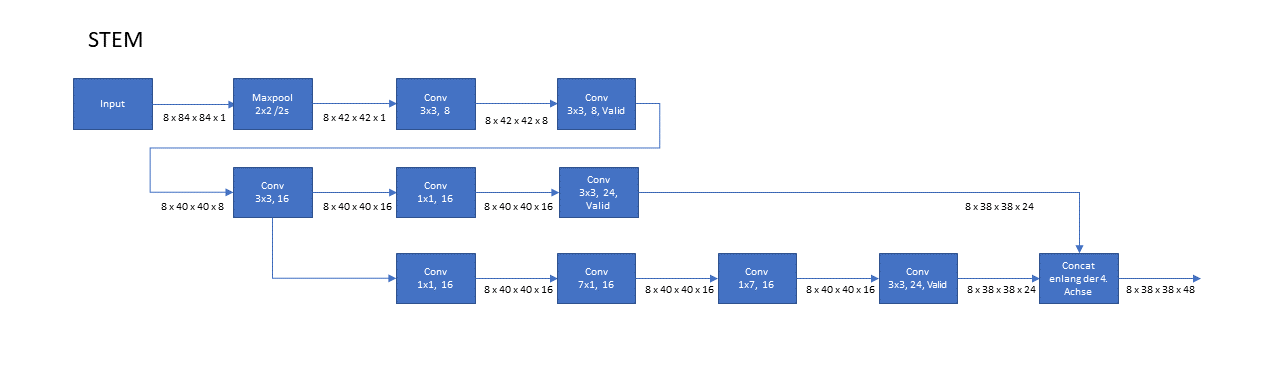
\includegraphics[scale=0.75]{pictures/Inception/STEM}
\label{fig:stem}
\end{sidewaysfigure}

Der STEM-Block aus Grafik \ref{fig:stem} bildet die Eingabeschicht der Architektur, welcher die ersten Berechnungen vollzieht und gleichzeitig der ersten Reduzierung der Bilddimensionen dient. In dieser Version sind nicht alle dimensionsreduzierenden Elemente des STEM-Blocks aus \textcite{DBLP:journals/corr/SzegedyIV16} enthalten, da die Eingabedimension der Daten dieser Arbeit wesentlich geringer ist, als die Bildgröße des ILSVRC 2012 Datensatzes (84x84 im Vergleich zu 299x299), somit ist eine weitere Reduktion der Daten vor Einführung des ersten Inception-Moduls nicht notwendig. Nach anfänglicher Verarbeitung durch einige Convolutional Layer, werden die Daten auf zwei Wegen weiterverarbeitet. Der erste Weg arbeitet mit quadratischen Filtergrößen, während der zweite Weg mit rechteckigen Filtergrößen in Reihe arbeitet. Beide Wege werden vor der Weitergabe an das nächste Modul entlang der Kanalachse (4. Achse) konkateniert, sodass aus den beiden Ausgaben mit Dimensionen 8x38x38x24 eine einzige Ausgabe mit 8x38x38x48 entsteht. Diese wird an das Inception-A-Modul weitergegeben. 

\begin{figure}[H]
\centering
\caption[Caption for LOF]{Übersicht der Inception V4-Module A,B und C}
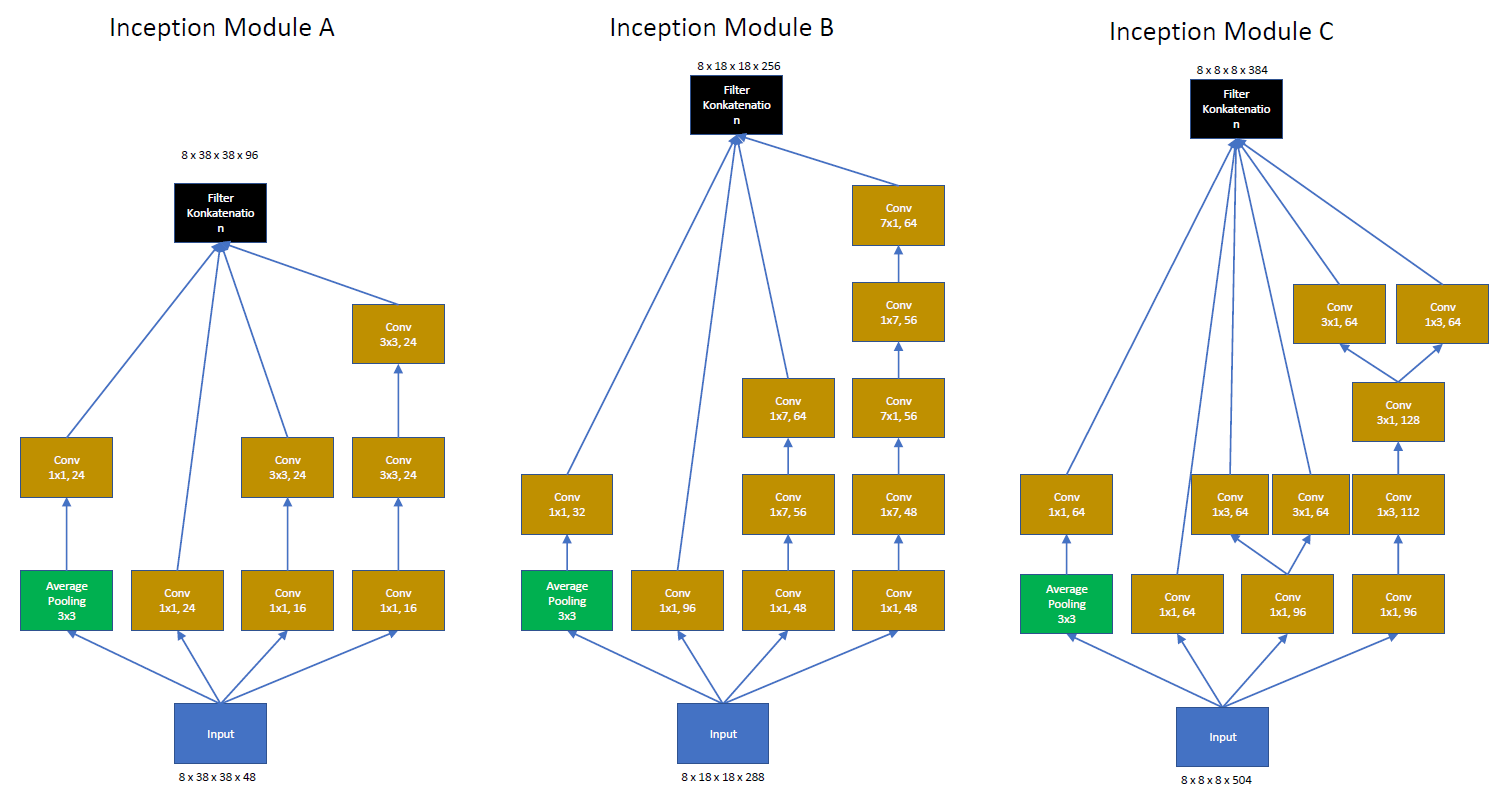
\includegraphics[scale=0.4]{pictures/Inception/InceptionABC}
\label{fig:incmod}
\end{figure}

Die Inception-Module (Grafik \ref{fig:incmod}) sind speziell für ihre Eingabegrößen angepasst. Alle Module spalten sich aus den Eingabedaten heraus in 4 Wege ab. In Modul C spalten sich zwei Wege erneut auf. Jedes Modul nutzt 1x1 Convolutional Layer um die Dimensionen der Eingabe vor der Verarbeitung oder Weitergabe zu reduzieren. Diese Layer findet man auf den drei rechten Wegen an erster Stelle und auf dem linken Weg nach dem Average Pooling in allen Modulen. Die Unterschiede zwischen den Modulen findet man hauptsächlich auf der rechten Seite aller Module, da sich die Convolutional Layer links lediglich durch die Filteranzahl unterscheiden. Auf der rechten Seite der Module lässt sich erkennen, dass Modul A auf symmetrische Filter setzt. Die Module B und C arbeiten jedoch mit asymmetrischen Filtern, welche meist entgegengesetzt angeordnet sind (3x1 folgt auf 1x3). Die rechten Wege in Modul B sind drei, bzw. fünf Layer tief und mit Filtern der Maße 1x7 und 7x1. In Modul C hingegen spalten sich die Wege nach einem und drei Layern auf und die Filter arbeiten mit 3x1 und 1x3 Layouts. Alle Module konkatenieren schlussendlich ihre vier bzw. sechs Verarbeitungspfade entlang der Kanalachse, bevor die Daten den nächsten Layer erreichen.

\begin{figure}[H]
\centering
\caption[Caption for LOF]{Übersicht der Inception V4-Reduktions-Module A und B}
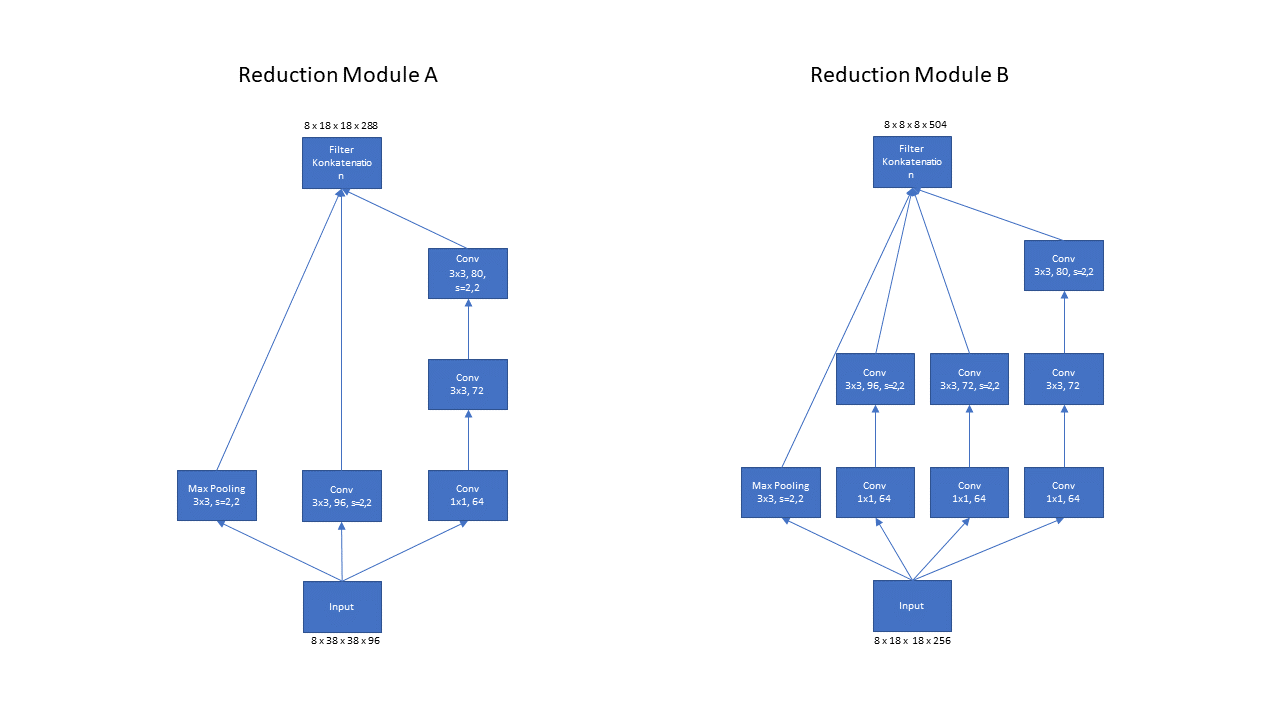
\includegraphics[scale=0.5]{pictures/Inception/Reduction}
\label{fig:incred}
\end{figure}

Zur Reduzierung der Bilddimensionen Höhe und Breite nutzt Inception Reduction-Module (Grafik \ref{fig:incred}). Beide Module nutzen sowohl Max-Pooling als auch Convolutional Layer mit Stride=2 um die Dimensionen der Eingabedaten entsprechend zu reduzieren. Reduction-A nutzt lediglich auf der rechten Seite des Moduls einen 1x1 Filter um die Dimensionen der Daten zu reduzieren. Bei Reduction-B kommt diese Methode bei den drei rechten Wegen zum Einsatz. In beiden Modulen wird mit 3x3 Filtern gearbeitet. Diese Filter reduzieren die Größe der Eingabedaten bzlg. Höhe $H^i$ und Breite $W^i$ wie folgt: $W^o = W^i / 2 - 1$ und $H^o = H^i / 2 - 1$. $W^o$ und $H^o$ stehen hier entsprechend für die Breite und Höhe der Ausgabe. Auch in den Reduction-Modulen werden die Ergebnisse der einzelnen Berechnungspfade zuletzt entlang der Kanalachse konkateniert. 

Tabelle \ref{tb:var_inc4} zeigt die einzelnen Module der Inception Architektur und ihre Variablenzahlen. In den Zahlen f\"ur Inception A, B und C sind die Variablen der Residual Network Verbindungen mit eingerechnet. 

\begin{table}
\centering
\caption{Inception V4: Auflistung der Variablenzahl.}
\begin{tabular}{@{}lr@{}}
\hline
Block & Parameter\\
\hline
STEM &  13.048\\
Inception A & 20.984\\
Reduction A & 182.144\\
Inception B & 265.464\\
Reduction B & 240.752\\
Inception C & 518.064\\
Fully-Connected & 786.496\\
Output Layer & 195\\
\hline
Summe Variablen & 2.027.147\\
\hline
\end{tabular}
\label{tb:var_inc4}
\end{table}

\subsection{Inception mit Squeeze-and-Excitation-Layer}

\textcite{DBLP:journals/corr/abs-1709-01507} hat Squezze-and-Excitation Layer eingeführt, um den Aspekt der Kanal Beziehungen zu untersuchen. Die Grundidee folgt dem Gedanken, dass unter den einzelnen Kanälen der Convolutional Layer Beziehungen modelliert werden können, welche es dem Netzwerk ermöglichen Feature Recalibration (zu Deutsch: \textit{Merkmal-Neukalibrierung}) auszuüben. Dieser Mechanismus ermöglicht es dem Netzwerk einzelne gewinnbringende Feature stärker zu gewichten und schwache Feature zu unterdrücken. Squeeze-and-Excitation Layer werden in der Arbeit von \textcite{DBLP:journals/corr/abs-1709-01507} nicht als eigenständige Bausteine eines Netzwerkes verstanden, sondern dienen als Erweiterung bestehender Architekturen. Daher wird in dieser Bachelorarbeit das Inception-Netzwerk, welches in Sektion \ref{sek:incv4} eingeführt wird, um diesen Layer erweitert. Grafik zeigt nach welchem Muster Squeeze-and-Excitation in Inception eingeführt werden kann. In der aktuellen Architektur werden die Squeeze-and-Excitation Layer jeweils nach den Inception Modulen angewendet. 

Squeeze-and-Excitation Layer bestehen -- wie in Grafik \ref{fig:sae} dargestellt -- aus vier zusätzlichen Elementen. Zunächst wird Global Average Pooling auf die Matrizen angewandt. Die Dimensionen der Ausgabe entsprechen in der Folge 1x1x1xAD, wobei AD für Ausgabedimension steht und gleich der Anzahl der Kanäle der Inception-Ausgabe ist. Als nächstes wird ein FCL genutzt für den ein neuer Hyperparameter Reduction-Ratio (RR, zu Deutsch: \textit{Reduktionsverhältnis}) eingeführt wird. Dieser Hyperparameter erlaubt es die Kapazität und Berechnungskosten der Squeeze-and-Excitation Layer zu beeinflussen, je höher der Wert gewählt ist, desto weniger Parameter fügen die Squeeze-and-Excitation Layer dem Netzwerk hinzu. Auf den FCL folgt eine ReLU-Aktivierung und dann erneut ein FCL, bei dem die Anzahl der Einheiten der AD entspricht. Das Ergebnis wird in die Ausgabe des Inception-Moduls integriert, indem die Werte des FCL kanalweise mit der Ausgabe multipliziert werden.  Die exakte Anzahl der Parameter dieser Version sind in Tabelle \ref{tb:var_inc_se} aufgelistet, wobei die Parameter der Squeeze-and-Excitation Layer in die Parameterzahl, der drei Inception Module eingerechnet sind.

\begin{figure}[H]
\centering
\caption[Caption for LOF]{Squeeze-and-Excitation Layer als Erweiterung der Inception-Module}
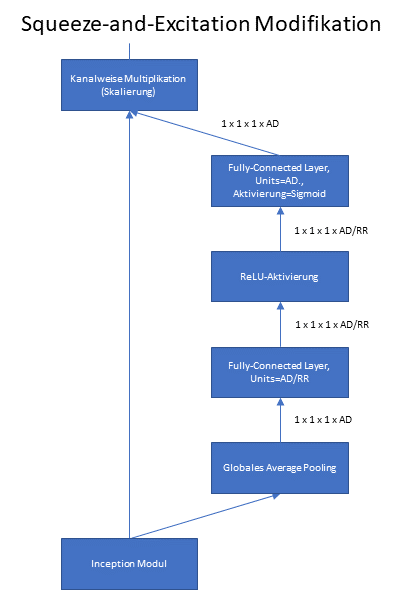
\includegraphics[scale=0.9]{pictures/Inception/SqueezeAndExcitation}
\label{fig:sae}
\end{figure}

\begin{table}
\centering
\caption{Inception-V4-SE-Net: Auflistung der Variablenzahl mit Squeeze-and-Excitation Layern.}
\begin{tabular}{@{}lr@{}}
\hline
Block & Parameter\\
\hline
STEM &  13.048\\
Inception A & 21.008\\
Reduction A & 182.144\\
Inception B & 224.568\\
Reduction B & 240.752\\
Inception C & 398.352\\
Fully-Connected & 786.496\\
Output Layer & 195\\
\hline
Summe Variablen & 1.866.563\\
\hline
\end{tabular}
\label{tb:var_inc_se}
\end{table}

\subsection{ResNet}
\label{sek:resnet}
ResNet ist eine von \textcite{He_2016} vorgestellte Architektur, welche sich Shortcut Connections (zu deutsch etwa: \textit{abkürzende Verbindungen}) zu nutze macht. Mit zunehmender Tiefe von CNNs wurde bei einigen Problemstellungen festgestellt, dass tiefere CNNs an Genauigkeit verlieren können, was im Allgemeinen der intuitiven Einschätzung widersprach, da man sich von dem Einsatz zusätzlicher Layer eine steigende Präzision erwartete. Da eine Evaluierung der Gradienten des entsprechenden CNNs das Vanishing Gradient Problem (zu deutsch etwa: \textit{verschwindende Gradienten Problem}) ausschloss, wurde die Vermutung aufgestellt, dass die Layer im CNN leichter sogenannte \textit{zero mappings} ($f(x) = 0$) lernen und daher nicht die Identitätsfunktion ($f(x) = x$). Als mögliche Lösung werden im Deep Resiual Neural Network shortcut connections eingefügt, welche ausschließlich als Identitätsfunktion dienen. 

Grafik \ref{fig:resnet} zeigt die Implementation eines ResNets mit acht Residual Blöcken. Die Eingabe wird zunächst von einem Convolutional Layer mit 7x7 Filtergröße und Stride=2 verarbeitet um die Dimensionen der Eingabe zu reduzieren. Nachfolgend werden diverse Residual Blöcke hintereinander gereiht. Die Residual Blöcke bestehen aus zwei Convolutional Layern mit einer Filtergröße von 3x3 und werden von einer Residual Connection überbrückt. Diese bildet in allen Blöcken mit Ausnahme von Block 6 die Identität der Eingabematrizen ab und wird nach den beiden Convolutional Layern hinzu addiert. Da Block 6 die Dimensionen in Höhe und Breite der Eingabe durch einen Stride-Parameter=2 reduziert und zugleich die Anzahl der Kanaldimensionen auf 128 erhöht, muss die Residual Connection mittels eines Convolutional Layers die gleichen Berechnungen vollziehen. Daher besteht in diesem Fall die Residual Connection aus einem Convolutional Layer mit Filtergröße 3x3 und Stride=2. Nach den Residual Blöcken werden die Daten wie bei Inception V4 mittels Average Pooling auf die Dimensionen 8x2x2x128 (Kanalanzahl) reduziert und danach von einem FCL mit 64 Einheiten weiterverarbeitet. Der Ausgabelayer wird von einem FCL mit drei Einheiten gebildet. Tabelle \ref{tb:resnet} listet die Anzahl der Parameter auf.

\begin{sidewaysfigure}
\centering
\caption[Caption for LOF]{ResNet mit acht Residual Blöcken}
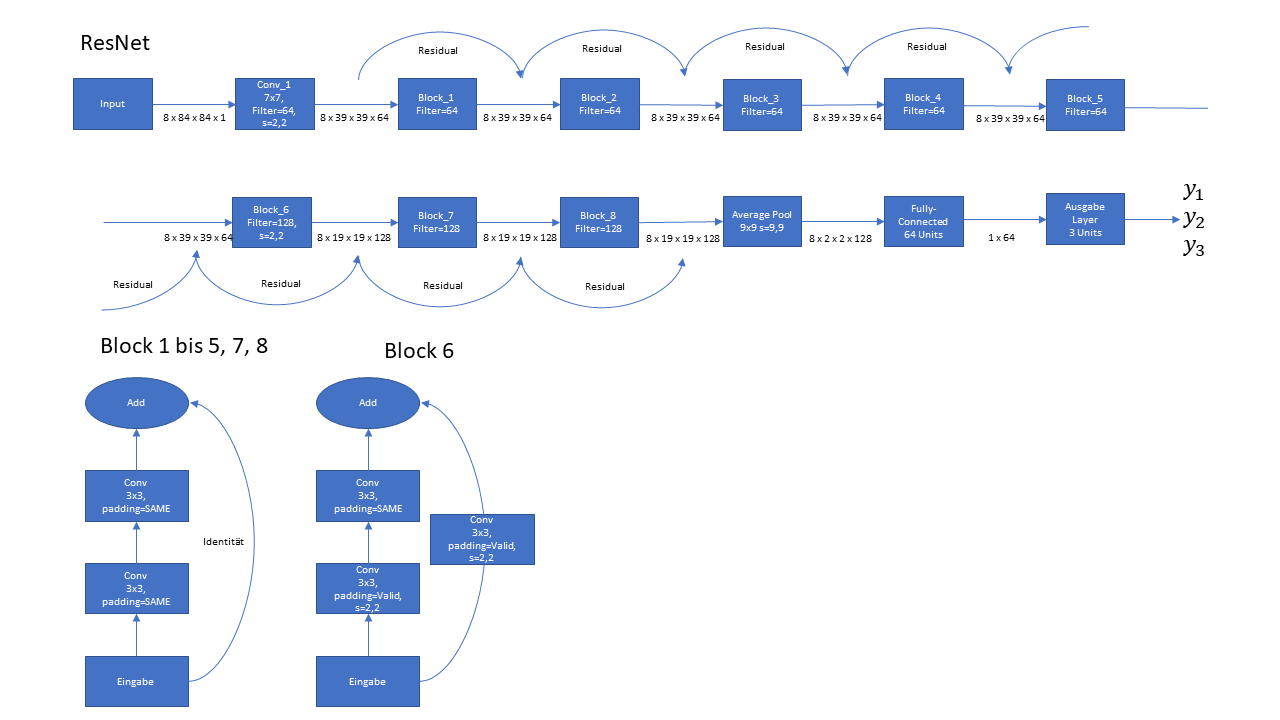
\includegraphics[scale=0.75]{pictures/Inception/ResNet}
\label{fig:resnet}
\end{sidewaysfigure}

\begin{table}
\centering
\caption{ResNet: Auflistung der Variablenzahl.}
\begin{tabular}{@{}lr@{}}
\hline
Block & Parameter\\
\hline
7x7 Conv &  3.328\\
Block 1 & 73.984\\
Block 2 & 73.984\\
Block 3 & 73.984\\
Block 4 & 73.984\\
Block 5 & 73.984\\
Block 6 & 295.552\\
Block 7 & 295.424\\
Block 8 & 295.680\\
FCL Units=64 & 262.208\\
Ausgabe Layer & 195\\
\hline
Summe Variablen & 1.522.307\\
\hline
\end{tabular}
\label{tb:resnet}
\end{table}


\section{Evaluation}

\subsection{Datengenerierung}
\label{datagen}

Der Vorgang der Datengenerierung wurde nach dem in Abbildung \ref{fig:overview2} aufgezeigten Schema implementiert. Durch die Verwendung einer Custom Map (zu Deutsch: \textit{benutzerdefinierten Karte}), eine durch den in StarCraft~II mitgelieferten Editor modifizierte Spielfläche, können die beiden Armeen mit zufällig zusammengestellten Einheiten-Konstellationen generiert werden. Zu Beginn des Gefechts werden beide Armeen am gegenseitigen Ende der Karte erzeugt. Bevor die Armeen den Kampf beginnen, wird der Spiel-Zustand (Spieler IDs, Höhenkarte, Einheitentyp, etc.) in Form von mehreren Matrix-Repräsentationen gespeichert. Sobald eine der beiden Seiten keine Einheiten mehr hat gilt die Schlacht als beendet und die Armee, welche noch über Einheiten verfügt wird als Sieger betrachtet. Das Ergebnis wird als Integer-Wert gespeichert und im späteren Verlauf des Trainings zu einem One-Hot-Vektor transformiert. 

Die Armeen werden zufällig generiert, der Generierungsprozess läuft wie folgt ab: Zunächst wird für beide Armeen eine Rasse gewürfelt. Die Rasse bestimmt welche Einheiten die Armee erzeugen darf. Im Folgenden wird für jede Einheit durch einen Zufallszahlen-Generator die Anzahl der maximal zu erzeugenden Einheiten ermittelt. Die Anzahl der Einheit, welche insgesamt von einer Armee erzeugt werden dürfen ist auf eine zufällige Grenze zwischen 10 und 50 begrenzt. Es werden daher alle Werte der einzelnen Einheiten so reduziert, dass die Gesamtzahl der Einheiten in einer Armee diese Grenze nicht überschreitet. Da bei zu großen Unterschieden in der Armeegröße die Klassifizierung zu einer trivialen Aufgabe wird, wurde zusätzlich eine Versorgungs-Grenze implementiert. In StarCraft~II ist die Versorgungsgrenzer ein Wert, welcher die Größe der Armee eines Spieler begrenzt. Diese Grenze wird in dem Kontext der Datengenerierung genutzt um nur jene Gefechte zu erzeugen, in denen der Unterschied der Einheiten-Versorgung beider Armeen kleiner ist als ein definierter Grenzwert (in diesem Fall 5).

Abbildung \ref{fig:overview1} zeigt den Generierungsprozess in Gänze. Die Custom Map aus StarCraft~II generiert ein Gefecht mit passender Differenz an Einheiten-Versorgung und lässt dieses nach speichern des Spielzustands austragen. Dieser Vorgang wird vor dem Beenden der Custom Map 25 Mal ausgeführt. Mit Beenden der Custom Map werden alle Vorgänge auf der Karte, als Replay (zu Deutsch: \textit{Wiederholung}) gespeichert. Ein Replay enthält somit 25 Gefechte, welche alle einzeln ausgewertet werden. 

Die Entscheidung mehrere Gefechte auf einmal zu generieren wurde getroffen, da die Custom Map bei jedem Start das Spiel neu laden muss und somit der zeitliche Overhead bei Einzelgenerierung der Replays wesentlich größer wäre. Die Anzahl der in einem Replay generierten Gefechte wurde auf 25 gesetzt, da bei zu vielen Iterationen der Gefechtsgenerierung die Replay-Datei zu groß wurde und das Spiel beim Schließen der Custom Map abstürzte. Der Absturz resultierte in jedem Fall in einem Datenverlust. Bei 25 Gefechten pro Replay liegt die Absturzrate derzeit immer noch bei ca. 50\%, jedoch resultierte das weitere Senken der Gefechte pro Replay nicht in einem stabileren Generationsprozess. 

Die Generierung der Gefechte findet auf der schnellsten Spieleinstellung statt, damit in gleicher Zeit mehr Gefechte simuliert werden können. Dadurch ist es aktuell möglich in einem Zeitraum von acht Stunden ca. 250 valide (500 Generierungen inklusive der Abstürze) Replays zu produzieren, welche nach der Feature Extraktion (Zeitaufwand erneut ca. drei bis vier Stunden) in 6250 Samples resultieren. 

\newpage
\begin{figure}[H]
\thispagestyle{empty}
\centering
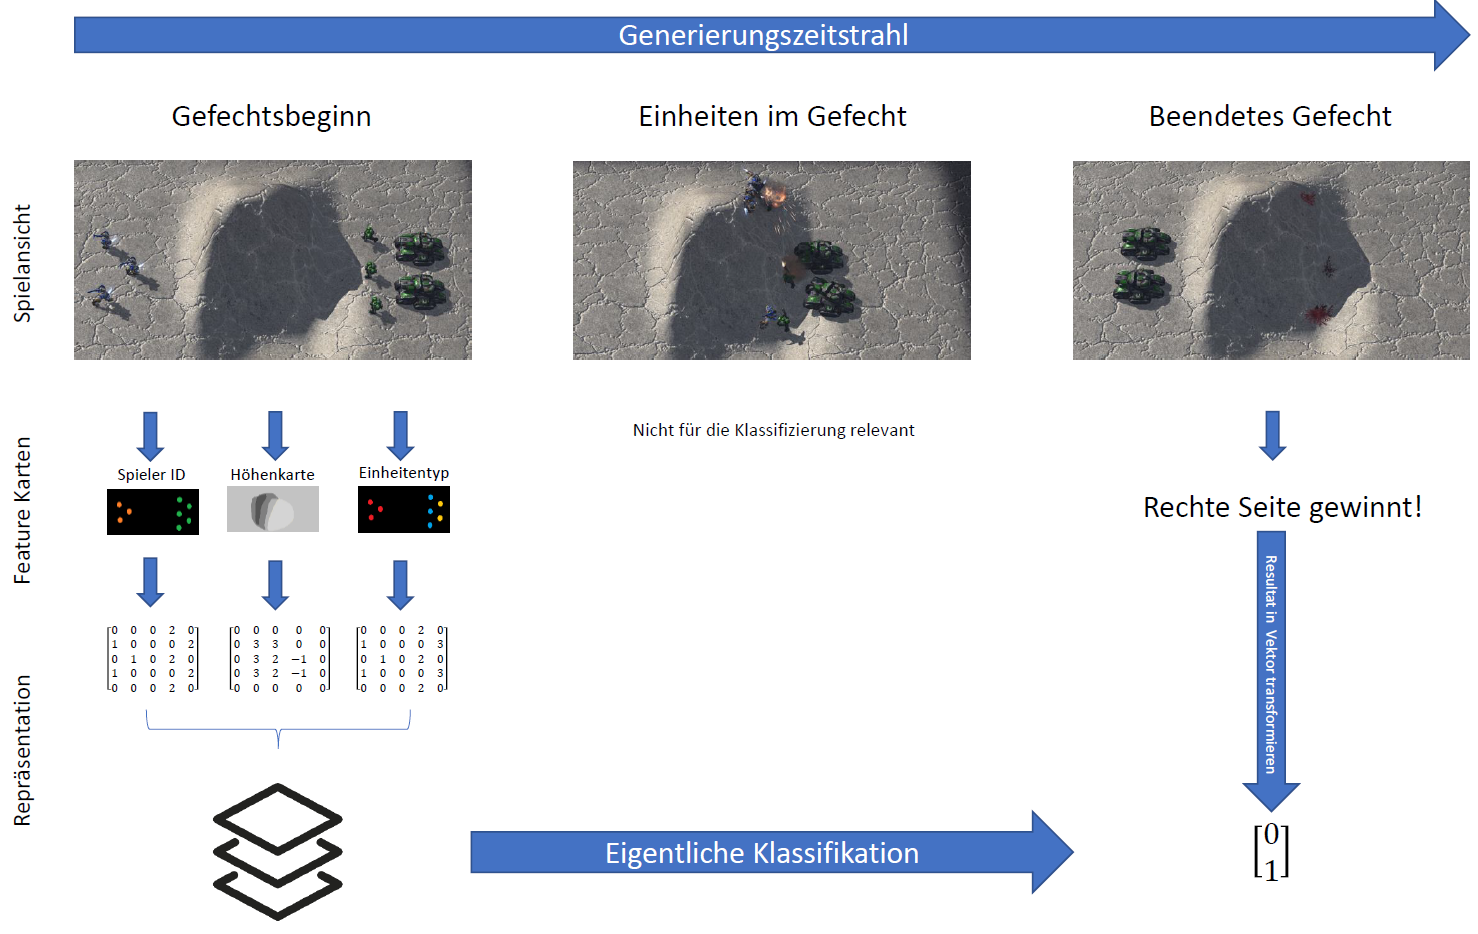
\includegraphics[angle=90,scale=0.6]{pictures/grafiken/Folie1}
\caption{Übersicht des Generierungsprozesses der Trainingsdaten}
\label{fig:overview2}
\end{figure}

\begin{figure}[H]
\thispagestyle{empty}
\centering
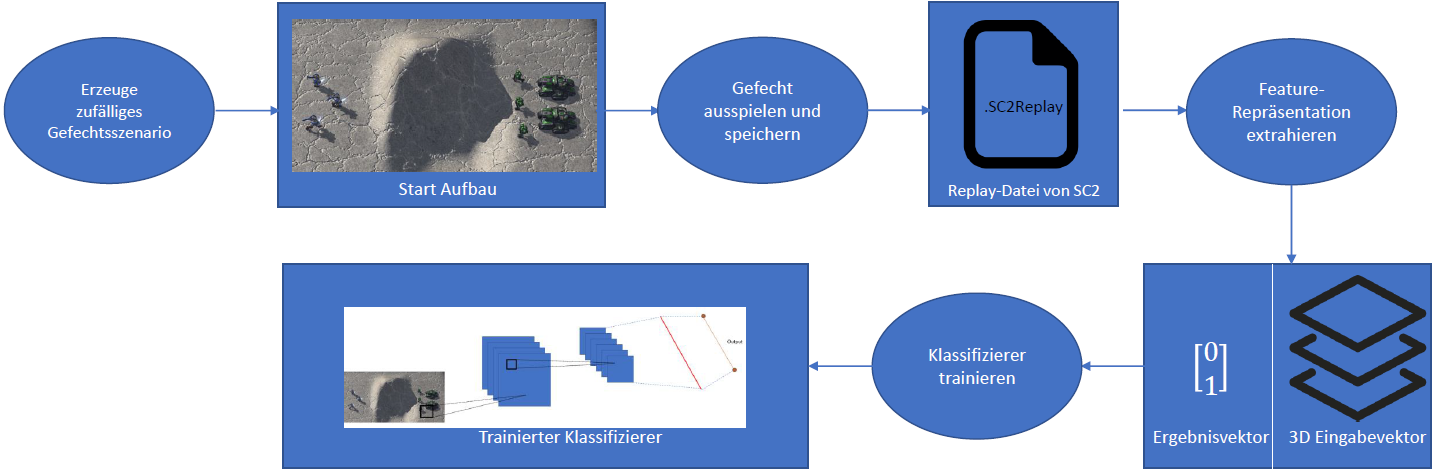
\includegraphics[angle=90,scale=0.6]{pictures/grafiken/Folie2}
\caption{Übersicht des Generierungsprozesses der Trainingsdaten}
\label{fig:overview1}
\end{figure}


\subsection{Resultate}
\label{Resultate}

\subsection{Auswertung}
\label{Auswertung}
\section{Konklusion}

Die Resultate der Arbeit zeigen, dass der Übertrag der Architekturen auf eine neue Domäne nur bedingt geglückt ist. Während das Overfitten der Architekturen während des Trainings aufzeigt, dass die Architekturen mit den Eingabedaten arbeiten und auf diesen lernen können, liegt die Performance der Architekturen hinter den Ergebnissen vorheriger Arbeiten. Die Architekturen generalisieren bisher nicht gut genug, besitzen jedoch die Möglichkeit die Trainingsdaten bis zu einer Accuracy von teilweise über 90\% vorherzusagen. Dieser Umstand kann bei besserer Generalisierung dazu beitragen, dass die Ergebnisse zukünftiger Architekturen besser ausfallen. Insgesamt weisen alle Architekturen zumindest bessere Ergebnisse als die naive Baseline auf. Anhand der Ergebnisse der Architekturen konnte weiterhin gezeigt werden, dass alle Netze Probleme mit der Vorhersage von Remis haben. Als mögliche Lösung könnten Remis im Anwendungsfall auch zu einer Niederlage evaluiert werden, da auch ein Remis in einer Wettkampfsituation kein erstrebenswerter Gefechtsausgang ist. Zudem ließ sich die These, dass Gefechte mit größeren Einheitenunterschieden einfacher vorherzusagen sind auch für die Vorhersage durch Neural Networks bestätigen. Die besten Leistungen zeigten die Architekturen Inception V4 auf den Testdaten (Accuracy: 0,63) und ResNet auf dem externen Datensatz (Accuracy: 0,62).

In weiteren Arbeiten kann der stärkere Einsatz von dreidimensionalen Convolutions untersucht werden. In den gelaufenen Trainings waren alle Convolutions mit einem Filter der Dimension mit Tiefe 1 konfiguriert. Eine Untersuchung, ob eine Filtertiefe $>1$ eine Steigerung der Accuracy liefert steht noch aus. Aufbauend auf variablen Größen der Filtertiefe könnte   eine Unterteilung nach semantischen Gemeinsamkeiten in kleinere Blöcke eine Steigerung der Performance mit sich bringen, indem man gezielt z.B. alle Feature Layer die Einheitenwerte betreffen zusammen evaluiert. So könnten die Layer Einheiten-Typ, Lebenspunkte und Schild zusammen verarbeitet werden und Layer, welche die Einheiten einem Spieler zuordnen im späteren Verlauf separat verrechnet werden.

In den Untersuchungen von \textcite{SnchezRuizGranados2015PredictingTO} zeigt dieser klar eine starke Verbesserung der Vorhersagegenauigkeit mit fortschreitendem Verlauf des Gefechts auf. Eine Untersuchung der Gefechte auf Basis einer Zeitreihe der ersten 5-10 Sekunden, könnte z.B. mit einem Long short-term memory network (LSTM-Network, zu Deutsch: \textit{langes Kurzzeitgedächtnis Netzwerk}) analysiert werden und damit die Accuracy der Vorhersage verbessern. 

Aktuell beziehen sich die Vorhersagen noch auf den Bildschirm, welcher dem Spieler zur Verfügung steht und finden basierend auf Daten von einem neutralen Beobachter statt, der alle Einheiten -- auch die unsichtbaren -- sehen kann. Als nächsten Schritt kann die Minimap einbezogen werden, welche einen Überblick über das gesamte Sichtfeld der Spieler liefert. Zusätzlich kann die Rolle eines Spieler eingenommen werden, der nur die Einheiten in seinem Sichtfeld sieht. Außerdem können Höhenunterschiede in die Custom Map eingebaut werden, welche die Ausgangssituation des Gefechts verändern. 

Einhergehend mit einer Erweiterung der Modelle kann die Performance mit der Implementation in einen Bot evaluiert und mit gängigen und bereits implementierten Entscheidungsalgorithmen verglichen werden. Unter Einbindung von Bots oder Scripts können die Modelle zusätzlich um den Einsatz von Fähigkeiten und das Nutzen von Micromanagement erweitert werden. 

\printbibliography
\end{document}